\documentclass[a4paper]{book}

\usepackage{bm}
\usepackage{caption}
\usepackage{enumitem}	% 定制enumerate标号
\usepackage{geometry}
\geometry{%
	left=2cm,%
	right=2cm,%
	top=2cm,%
	bottom=2cm,%
	bindingoffset=0cm}
\usepackage[none]{hyphenat}	% 阻止长单词分在两行
\usepackage{mathrsfs}	% 提供\mathscr字体
\usepackage[version=4]{mhchem}

\RequirePackage[many]{tcolorbox}
\tcbset{
    boxed title style={colback=magenta},
	breakable,
	enhanced,
	sharp corners,
	attach boxed title to top left={yshift=-\tcboxedtitleheight,  yshifttext=-.75\baselineskip},
	boxed title style={boxsep=1pt,sharp corners},
    fonttitle=\bfseries\sffamily,
}

\definecolor{skyblue}{rgb}{0.54, 0.81, 0.94}

\newtcolorbox[auto counter, number within=chapter, number format=\arabic]{exercise}[1][]{
    title={Exercise~\thetcbcounter},
    colframe=skyblue,
    colback=skyblue!12!white,
    boxed title style={colback=skyblue},
    overlay unbroken and first={
        \node[below right,font=\small,color=skyblue,text width=.8\linewidth]
        at (title.north east) {#1};
    }
}

\newtcolorbox[auto counter, number within=chapter, number format=\arabic]{solution}[1][]{
%    top=2ex,
%    boxrule=0pt,
%    leftrule=1.4pt,
    title={Solution~\thetcbcounter},
    colframe=teal!60!green,
    colback=green!12!white,
    boxed title style={colback=teal!60!green},
    overlay unbroken and first={
        \node[below right,font=\small,color=red,text width=.8\linewidth]
        at (title.north east) {#1};
    }
}

\newcommand{\AO}{{\rm AO}}
\newcommand{\Heff}{H^{\rm eff,\pi}}
\newcommand{\orb}[1]{{\rm #1}}
\newcommand{\orbs}{\orb{s}}
\newcommand{\orbp}{\orb{p}}
\newcommand{\orbd}{\orb{d}}
\newcommand{\orbf}{\orb{f}}

\newcommand\Figref[1]{Fig \ref{#1}}
\newcommand\Tableref[1]{Table \ref{#1}}

\setlength{\tabcolsep}{4pt}
\renewcommand{\arraystretch}{1.1}

\begin{document}

	\setcounter{chapter}{11}

	\begin{exercise}
		Determine the irreducible representations of $\mathscr{T}_{\rm d}$ to which f-orbitals belong.
	\end{exercise}

	\begin{solution}

		Firstly, the information of seven (un-normalized) f-orbitals is listed below and they are marked in my symbols.
		\begin{center}
		\begin{tabular}{ccc}\hline
		angular function &	f-orbital symfol & 	my symbol \\ \hline
	$\sin\theta\cos\phi(5\sin^2\theta\cos^2\phi-3)$ &	$\orbf_{x(5x^2-3r^2)}$ or $\orbf_{x^3}$ & $f_1$ \\
	$\sin\theta\sin\phi(5\sin^2\theta\sin^2\phi-3)$ &	$\orbf_{y(5y^2-3r^2)}$ or $\orbf_{y^3}$ & $f_2$ \\
	$5\cos^3\theta - 3\cos\theta$ &	$\orbf_{z(5z^2-3r^2)}$ or $\orbf_{z^3}$ & $f_3$ \\
	$\sin\theta\cos\phi(\cos^2\theta-\sin^2\theta\sin^2\phi)$ &	$\orbf_{x(z^2-y^2)}$ & $f_4$ \\
	$\sin\theta\sin\phi(\cos^2\theta-\sin^2\theta\cos^2\phi)$ &	$\orbf_{y(z^2-x^2)}$ & $f_5$ \\
	$\sin^2\theta\cos\phi\cos2\phi$ & $\orbf_{z(x^2-y^2)}$ & $f_6$ \\
	$\sin^2\theta\cos\phi\sin2\phi$ & $\orbf_{xyz}$ & $f_7$ \\\hline
		\end{tabular}
		\end{center}
		
		\begin{center}
		\begin{tabular}{cccc}
			\begin{minipage}[t]{0.22\linewidth}
			\centering
			\setlength{\abovecaptionskip}{0.5em}
			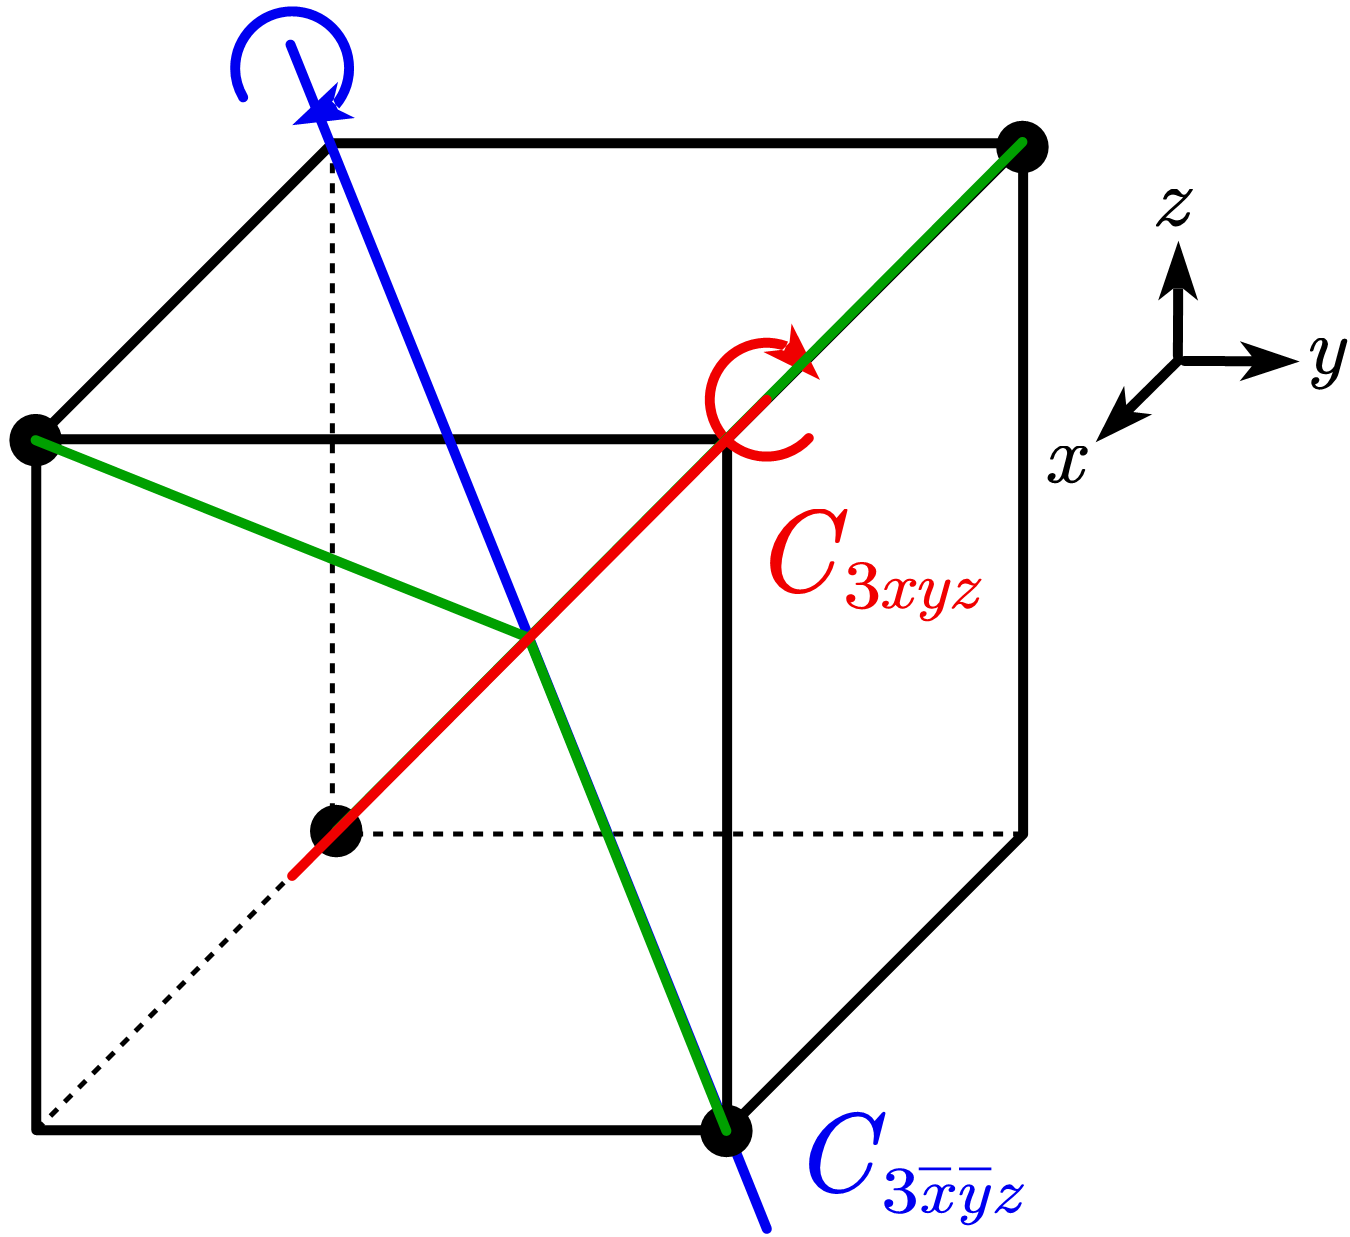
\includegraphics[scale=1]{./structures/exercise_1/f-orbitals_C3.png}
			\captionof*{figure}{class $\{C_3\}$}
			\end{minipage} & 
			\begin{minipage}[t]{0.22\linewidth}
			\setlength{\abovecaptionskip}{0.5em}
			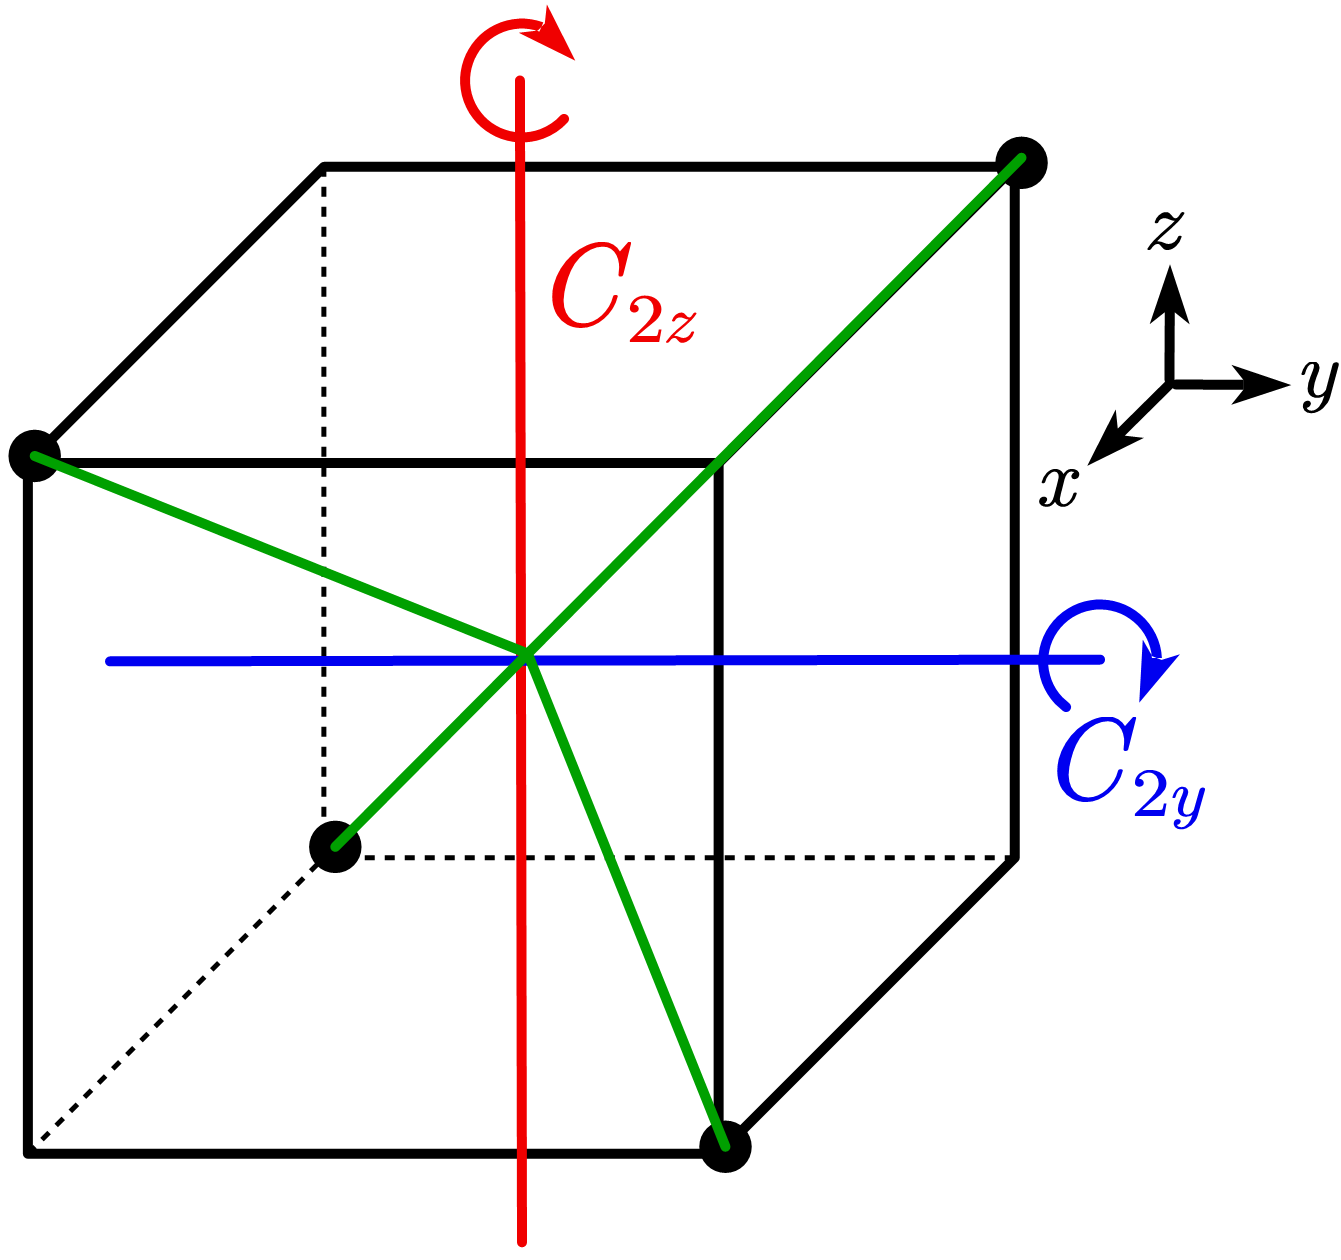
\includegraphics[scale=1]{./structures/exercise_1/f-orbitals_C2.png}
			\captionof*{figure}{class $\{C_2\}$}
			\end{minipage} &
			\begin{minipage}[t]{0.22\linewidth}
			\centering
			\setlength{\abovecaptionskip}{0.5em}
			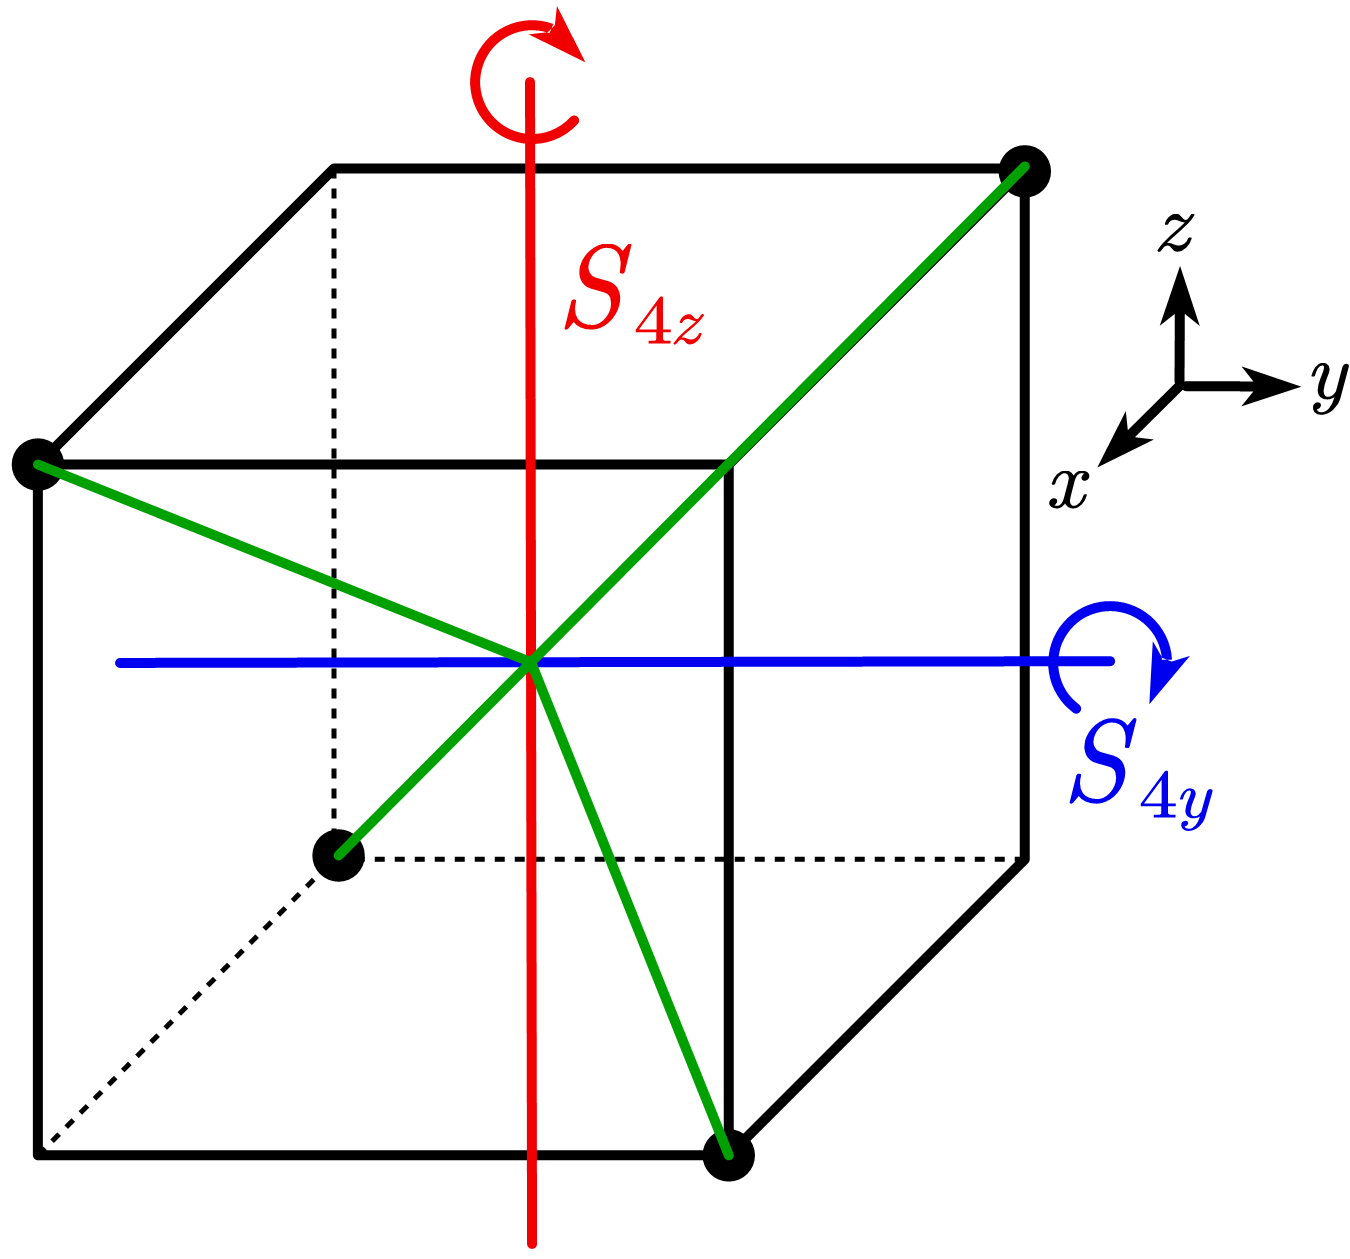
\includegraphics[scale=1]{./structures/exercise_1/f-orbitals_S4.png}
			\captionof*{figure}{class $\{S_4\}$}
			\end{minipage} & 
			\begin{minipage}[t]{0.22\linewidth}
			\setlength{\abovecaptionskip}{0.5em}
			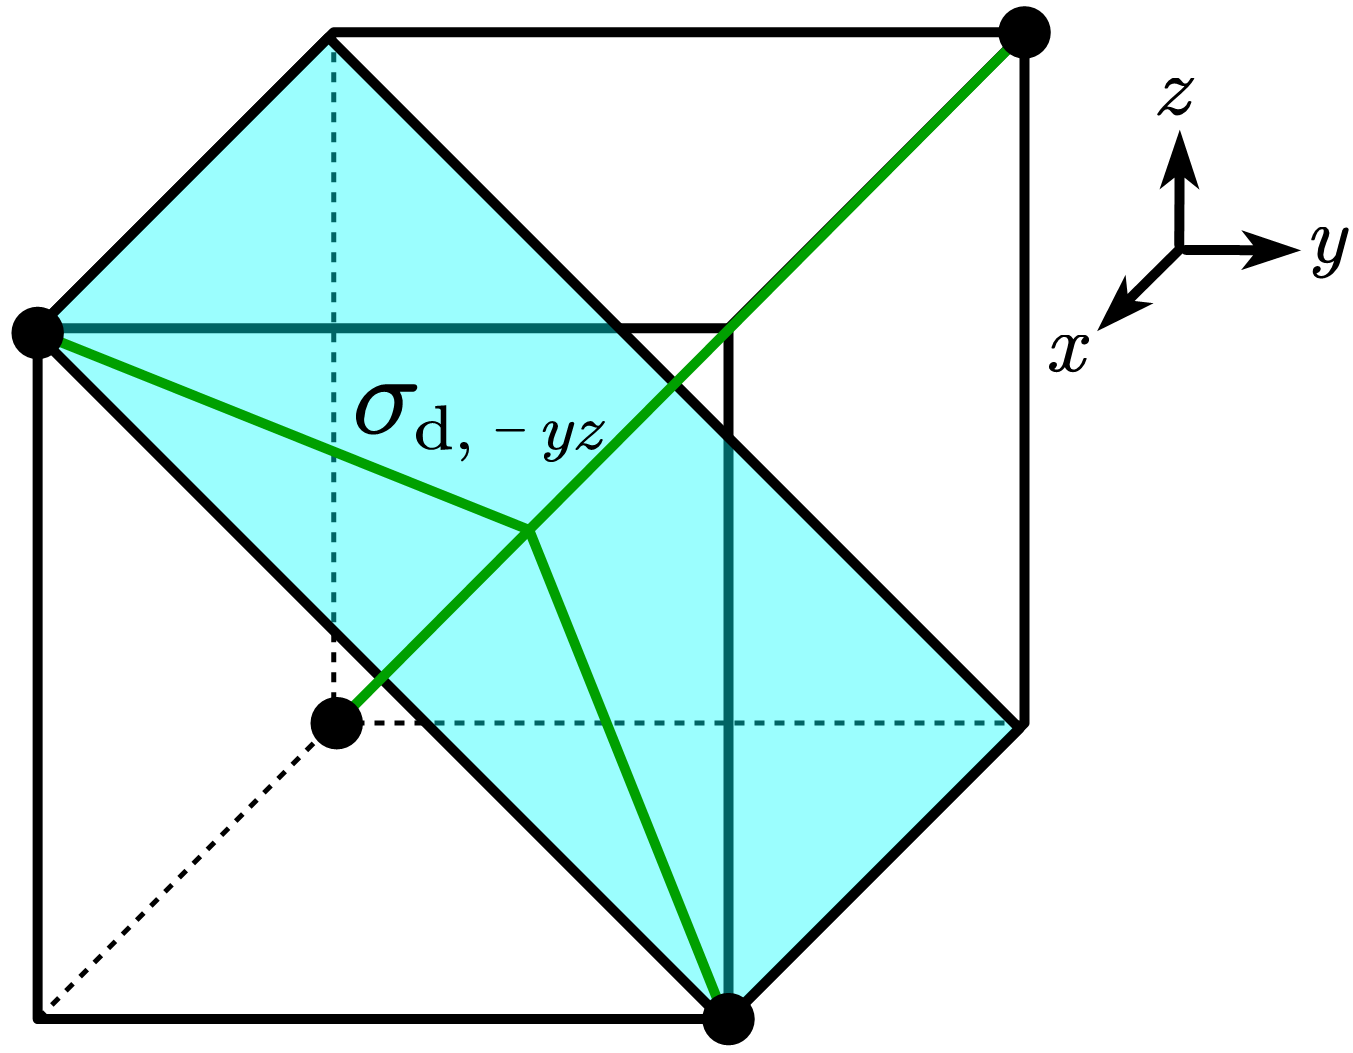
\includegraphics[scale=1]{./structures/exercise_1/f-orbitals_sigma.png}
			\captionof*{figure}{class $\{\sigma_{\rm d}\}$}
			\end{minipage}
		\end{tabular}				
		\captionof{figure}{aaaaaaa}
		\end{center}
		
		Then, the definition of all operation $R$ is demonstrated below, and they are classified according to their classes. Note that $R(x^\prime,y^\prime,z^\prime)$ means that $x$, $y$, $z$ are converted to $x^\prime$, $y^\prime$, $z^\prime$, respectively.
		\begin{itemize}

		\item class $E$
		
		There is only one element, i.e. identical operation $E$, which is $E(x,y,z)$.
		
		\item class $C_3$

		There are 8 elements, whose information is listed below. \vspace{-1em}
		\begin{center}
		\begin{tabular}{c|c} \hline
			$C_{3xyz}(y,z,x)$	& rotate $\frac {2\pi}3$ clockwise around $\bm{i+j+k}$\\
			$C^{-1}_{3\bar x\bar yz}(z,x,y)$ & rotate $\frac {4\pi}3$ clockwise around $\bm{i+j+k}$ \\
			$C_{3\bar x\bar yz}(y,\bar z,\bar x)$ &  rotate $\frac {2\pi}3$ clockwise around $\bm{-i-j+k}$ \\
			$C^{-1}_{3\bar x\bar yz}(\bar z,x,\bar y)$ & rotate $\frac {4\pi}3$ clockwise around $\bm{-i-j+k}$ \\
			$C_{3\bar x y \bar z}(\bar y, \bar z,x)$ &  rotate $\frac {2\pi}3$ clockwise around $\bm{-i+j-k}$ \\
			$C^{-1}_{3\bar x y \bar z}(z, \bar x,\bar y)$ & rotate $\frac {4\pi}3$ clockwise around $\bm{-i+j-k}$ \\
			$C_{3x\bar y \bar z}(\bar y, z,\bar x)$ &  rotate $\frac {2\pi}3$ clockwise around $\bm{i-j-k}$ \\
			$C^{-1}_{3x\bar y \bar z}(\bar z,\bar x,y)$ & rotate $\frac {4\pi}3$ clockwise around $\bm{i-j-k}$ \\ \hline
		\end{tabular}
		\end{center}
		
		\item class $C_2$

		There are 3 elements, whose information is listed below. \vspace{-1em}
		\begin{center}
		\begin{tabular}{c|c} \hline
			$C_{2x}(x,\bar y, \bar z)$	& rotate $\pi$ clockwise around $x$-axis\\
			$C_{2y}(\bar x, y, \bar z)$	& rotate $\pi$ clockwise around $y$-axis\\
			$C_{2z}(\bar x,\bar y, z)$	& rotate $\pi$ clockwise around $z$-axis\\ \hline
		\end{tabular}
		\end{center}
		
		\item class $S_4$

		There are 6 elements, whose information is listed below. \vspace{-1em}
		\begin{center}
		\begin{tabular}{c|c} \hline
			$S_{4x}(\bar x,\bar z, y)$	& rotate $\frac\pi2$ clockwise around $x$-axis and then perform horizontal mirror reflection\\
			$S^3_{4x}(\bar x, z, \bar y)$	& rotate $\frac{3\pi}2$ clockwise around $x$-axis and then perform horizontal mirror reflection\\
			$S_{4y}(z, \bar y, \bar x)$	& rotate $\frac\pi2$ clockwise around $y$-axis and then perform horizontal mirror reflection\\
			$S^3_{4y}(\bar z, \bar y, x)$ & rotate $\frac{3\pi}2$ clockwise around $y$-axis and then perform horizontal mirror reflection\\
			$S_{4z}(\bar y, x, \bar z)$	& rotate $\frac\pi2$ clockwise around $z$-axis and then perform horizontal mirror reflection\\
			$S^3_{4z}(y, \bar x, \bar z)$	& rotate $\frac{3\pi}2$ clockwise around $z$-axis and then perform horizontal mirror reflection\\ \hline
		\end{tabular}
		\end{center}
		
		\item class $\sigma_{\rm d}$

		There are 6 elements, whose information is listed below. \vspace{-1em}
		\begin{center}
		\begin{tabular}{c|c} \hline
			$\sigma_{{\rm d},yz}(x, z, y)$ & perform mirror reflection about the $y-z=0$ plane \\
			$\sigma_{{\rm d},-yz}(x, \bar z, \bar y)$	& perform mirror reflection about the $y+z=0$ plane \\
			$\sigma_{{\rm d},xz}(z, y, x)$ & perform mirror reflection about the $x-z=0$ plane \\
			$\sigma_{{\rm d},-xz}(\bar z, y, \bar x)$	& perform mirror reflection about the $x+z=0$ plane \\
			$\sigma_{{\rm d},xy}(y, x, z)$ & perform mirror reflection about the $x-y=0$ plane \\
			$\sigma_{{\rm d},-xy}(\bar y, \bar x, z)$	& perform mirror reflection about the $x+y=0$ plane \\ \hline
		\end{tabular}
		\end{center}

		\end{itemize}				
		
		Next, the result of the transformation of these orbitals under $O_R$ is listed below. \vspace{-0.5em}
		\begin{center}
		\begin{tabular}{ccccccccccccc} \hline
			element & $E$ & $C_{3xyz}$ & $C^{-1}_{3xyz}$ & $C_{3\bar x \bar y z}$ & $C^{-1}_{3\bar x \bar yz}$ & $C_{3\bar x y \bar z}$ & $C^{-1}_{3\bar x y \bar z}$ &  $C_{3 x\bar y \bar z}$ & $C^{-1}_{3x\bar y \bar z}$ & $C_{2x}$ & $C_{2y}$ & $C_{2z}$ \\ \hline
			$f_1$	&	$f_1$	&	$f_2$	&	$f_3$	&	$f_2$	&	$-f_3$	&	$-f_3$	&	$-f_2$	&	$f_3$	&	$-f_2$	&	$f_1$	&	$-f_1$	&	$-f_1$	\\
			$f_4$	&	$f_4$	&	$-f_5$	&	$-f_6$	&	$-f_5$	&	$f_6$	&	$f_5$	&	$-f_6$	&	$f_5$	&	$f_6$	&	$f_4$	&	$-f_4$	&	$-f_4$	\\
			$f_7$	&	$f_7$	&	$f_7$	&	$f_7$	&	$f_7$	&	$f_7$	&	$f_7$	&	$f_7$	&	$f_7$	&	$f_7$	&	$f_7$	&	$f_7$	&	$f_7$	\\ \hline
			element & $S_{4x}$ & $S^3_{4x}$ & $S_{4y}$ & $S^3_{4y}$ & $S_{4z}$ & $S^{3}_{4z}$ & $\sigma_{{\rm d},yz}$ &  $\sigma_{{\rm d},-yz}$ & $\sigma_{{\rm d},xz}$ & $\sigma_{{\rm d},-xz}$ & $\sigma_{{\rm d},xy}$ & $\sigma_{{\rm d},-xy}$ \\ \hline
			$f_1$	&	$-f_1$	&	$-f_1$	&	$f_3$	&	$-f_3$	&	$-f_2$	&	$f_2$	&	$f_1$	&	$f_1$	&	$f_3$	&	$-f_3$	&	$f_2$	&	$-f_2$	\\
			$f_4$	&	$f_4$	&	$f_4$	&	$f_6$	&	$-f_6$	&	$-f_5$	&	$f_5$	&	$-f_4$	&	$-f_4$	&	$f_6$	&	$-f_6$	&	$f_5$	&	$-f_5$	\\
			$f_7$	&	$f_7$	&	$f_7$	&	$f_7$	&	$f_7$	&	$f_7$	&	$f_7$	&	$f_7$	&	$f_7$	&	$f_7$	&	$f_7$	&	$f_7$	&	$f_7$	\\ \hline
		\end{tabular}
		\end{center}
		
		Here, we check the character table of the point group $\mathscr{T}_{\rm d}$, \vspace{-0.5em}
		\begin{center}
		\begin{tabular}{cccccccc}\hline
	$\mathscr{T}_{\rm d}$ & $E$ & $8C_3$ &	$3C_2$	& $6S_4$	&	$6\sigma_{\rm d}$ &		&	\\ \hline
		$A_1$	&	1	&	1	&	1	&	1	&	1	&	& $x^2+y^2+z^2$	\\
		$A_2$	&	1	&	1	&	1	&	-1	&	-1	&	&	\\
		$E$		&	2	&	-1	&	2	&	0	&	0	&	& ($2z^2-x^2-y^2$, $x^2-y^2$)	\\
		$T_1$	&	3	&	0	&	-1	&	1	&	-1	& ($R_x$, $R_y$, $R_z$)	& 	\\
		$T_2$	&	3	&	0	&	-1	&	-1	&	1	& ($x$, $y$, $z$)	&	($xy$, $xz$, $yz$) 	\\ \hline
		\end{tabular}
		\end{center}
		and we find the character below for $\Gamma^{rm hyb}$ for the $\mathscr{T}_{\rm d}$ point group.
		\begin{center}
		\begin{tabular}{cccccc} \hline
			$\mathscr{T}_{\rm d}$ & $E$ & $8C_3$ &	$3C_2$	& $6S_4$	&	$6\sigma_{\rm d}$	\\ \hline
			$\chi^{\rm hyb}(C_i)$ & 7 & 1 & -1 & 1 & 1 \\\hline
		\end{tabular}
		\end{center}
		
		We can calculate the reduction of representation $\Gamma^{\rm hyb}$,
		\begin{align*}
		a_1 &= \frac{1}{24} [ 1 \times 7 \times 1 + 8 \times 1 \times 1 + 3 \times (-1) \times 1 + 6 \times 1 \times 1 + 6 \times 1 \times 1 ] = 1 ,\\
		a_2 &= \frac{1}{24} [ 1 \times 7 \times 1 + 8 \times 1 \times 1 + 3 \times (-1) \times 1 + 6 \times 1 \times (-1) + 6 \times 1 \times (-1) ] = 0, \\
		e &= \frac{1}{24} [ 1 \times 7 \times 2 + 8 \times 1 \times (-1) + 3 \times (-1) \times 2 + 6 \times 1 \times 0 + 6 \times 1 \times 0 ] = 0, \\
		t_1 &= \frac{1}{24} [ 1 \times 7 \times 3 + 8 \times 1 \times 0 + 3 \times (-1) \times (-1) + 6 \times 1 \times 1 + 6 \times 1 \times (-1) ] = 1 ,\\
		t_2 &= \frac{1}{24} [ 1 \times 7 \times 3 + 8 \times 1 \times 0 + 3 \times (-1) \times (-1) + 6 \times 1 \times (-1) + 6 \times 1 \times 1 ] = 1 ,
		\end{align*}
		and we obtain
		\begin{equation}
			\Gamma^{\rm hyb} = \Gamma^{A_1} \oplus \Gamma^{T_1} \oplus \Gamma^{T_2}.
		\end{equation}
		
		For simplification, we summarize the operations of the same classes.
		\begin{center}
		\begin{tabular}{cccccc}\hline
	$\mathscr{T}_{\rm d}$ & $O_E$ & $\sum_{k=1}^8 O_{C_{3k}}$ & $\sum_{k=1}^3 O_{C_{2k}}$	& $\sum_{k=1}^6 O_{S_{4k}}$	&	$ \sum_{k=1}^6 O_{\sigma_{{\rm d},k}}$	\\ \hline
		$f_1$	&	$f_1$	&	0	&	$-f_1$	&	$-2f_1$	&	$2f_1$	\\
		$f_4$	&	$f_4$	&	0	&	$-f_4$	&	$2f_4$	&	$-2f_4$	\\
		$f_7$	&	$f_7$	&	$8f_7$	&	$3f_7$	&	$6f_7$	&	$6f_7$	\\ \hline
		\end{tabular}
		\end{center}
		
		\begin{align*}
		P^{A_1} f_1 &= ( 1 \times O_E + 1 \times \sum_{k=1}^8 O_{C_{3k}} + 1 \times \sum_{k=1}^3 O_{C_{2k}} + 1 \times \sum_{k=1}^6 O_{S_{4k}} + 1 \times \sum_{k=1}^6 O_{\sigma_{{\rm d},k}} ) f_1 = 0, \\
		P^{A_2} f_1 &= ( 1 \times O_E + 1 \times \sum_{k=1}^8 O_{C_{3k}} + 1 \times \sum_{k=1}^3 O_{C_{2k}} + (-1) \times \sum_{k=1}^6 O_{S_{4k}} + (-1) \times \sum_{k=1}^6 O_{\sigma_{{\rm d},k}} ) f_1 = 0, \\
		P^E f_1 &= ( 2 \times O_E + (-1) \times \sum_{k=1}^8 O_{C_{3k}} + 2 \times \sum_{k=1}^3 O_{C_{2k}} + 0 \times \sum_{k=1}^6 O_{S_{4k}} + 0 \times \sum_{k=1}^6 O_{\sigma_{{\rm d},k}} ) f_1 = 0, \\
		P^{T_1} f_1 &= ( 3 \times O_E + 0 \times \sum_{k=1}^8 O_{C_{3k}} + (-1) \times \sum_{k=1}^3 O_{C_{2k}} + 1 \times \sum_{k=1}^6 O_{S_{4k}} + (-1) \times \sum_{k=1}^6 O_{\sigma_{{\rm d},k}} ) f_1 = 0, \\
		P^{T_2} f_1 &= ( 3 \times O_E + 0 \times \sum_{k=1}^8 O_{C_{3k}} + (-1) \times \sum_{k=1}^3 O_{C_{2k}} + (-1) \times \sum_{k=1}^6 O_{S_{4k}} + 1 \times \sum_{k=1}^6 O_{\sigma_{{\rm d},k}} ) f_1 = 8f_1. \\
		\end{align*}
		Thus, $f_1$ belongs to $T_2$, which is a three-dimentional irreducible representation. With
		\begin{equation*}
			C_{3xyz} f_1 = f_2, \quad C^{-1}_{3xyz} f_1 = f_3,
		\end{equation*}
		we conclude that $f_1$, $f_2$ and $f_3$ belong to $T_2$.
		
		Similarly, we note 
		\begin{equation*}
		P^{A_1} f_4 = 0, \quad	P^{A_2} f_4 = 0, \quad P^E f_4 = 0, \quad P^{T_1} f_4 = 8f_4, \quad P^{T_2} f_4 = 0.
		\end{equation*}
		So $f_4$ belongs to $T_1$. Besides, with
		\begin{equation*}
			C_{3xyz} f_4 = -f_5, \quad C^{-1}_{3xyz} f_4 = -f_6,
		\end{equation*}				
		we can also conclude that $f_4$, $f_5$ and $f_6$ belong to the same three-dimentional irreducible representation $T_1$.
		\begin{equation*}
		P^{A_1} f_7 = 24f_7, \quad	P^{A_2} f_7 = 0, \quad P^E f_7 = 0, \quad P^{T_1} f_7 = 0, \quad P^{T_2} f_7 = 0.
		\end{equation*}
		Thus, we conclude that $f_7$ belongs to the one-dimentional irreducible representation $A_1$.
		
		In conclusion, we find 
		\begin{itemize}
		
		\item $f_1 \equiv \orbf_{x(5x^2-3r^2)}$, $f_2 \equiv \orbf_{y(5y^2-3r^2)}$ and $f_3 \equiv \orbf_{z(5z^2-3r^2)}$ belong to the three-dimentional irreducible representation $T_2$,

		\item $f_4 \equiv \orbf_{x(z^2-y^2)}$, $f_5 \equiv \orbf_{y(z^2-x^2)}$ and $f_6 \equiv \orbf_{z(x^2-y^2)}$ belong to the three-dimentional irreducible representation $T_1$,
		
		\item $f_7 \equiv \orbf_{xyz}$ belongs to the one-dimentional irreducible representation $A_1$.

		\end{itemize}				
		 
		
	\end{solution}
	
	\begin{exercise}
		Show that for a molecule of octahedral symmetry the $\sigma$-bonding hybrid orbitals on the central atom are composed of six atomic orbitals: $\orbs$, $\orbp_x$, $\orbp_y$, $\orbp_z$, $\orbd_{z^2}$ and $\orbd_{x^2-y^2}$.
	\end{exercise}

	\begin{solution}
		
		The structure of a general molecule $\ce{AB6}$ of octahedral symmetry is shown in \Figref{fig:octahedral}.
		
		
		\begin{minipage}[t]{1.0\linewidth}
		\begin{center}
		\setlength{\abovecaptionskip}{0.5em}
		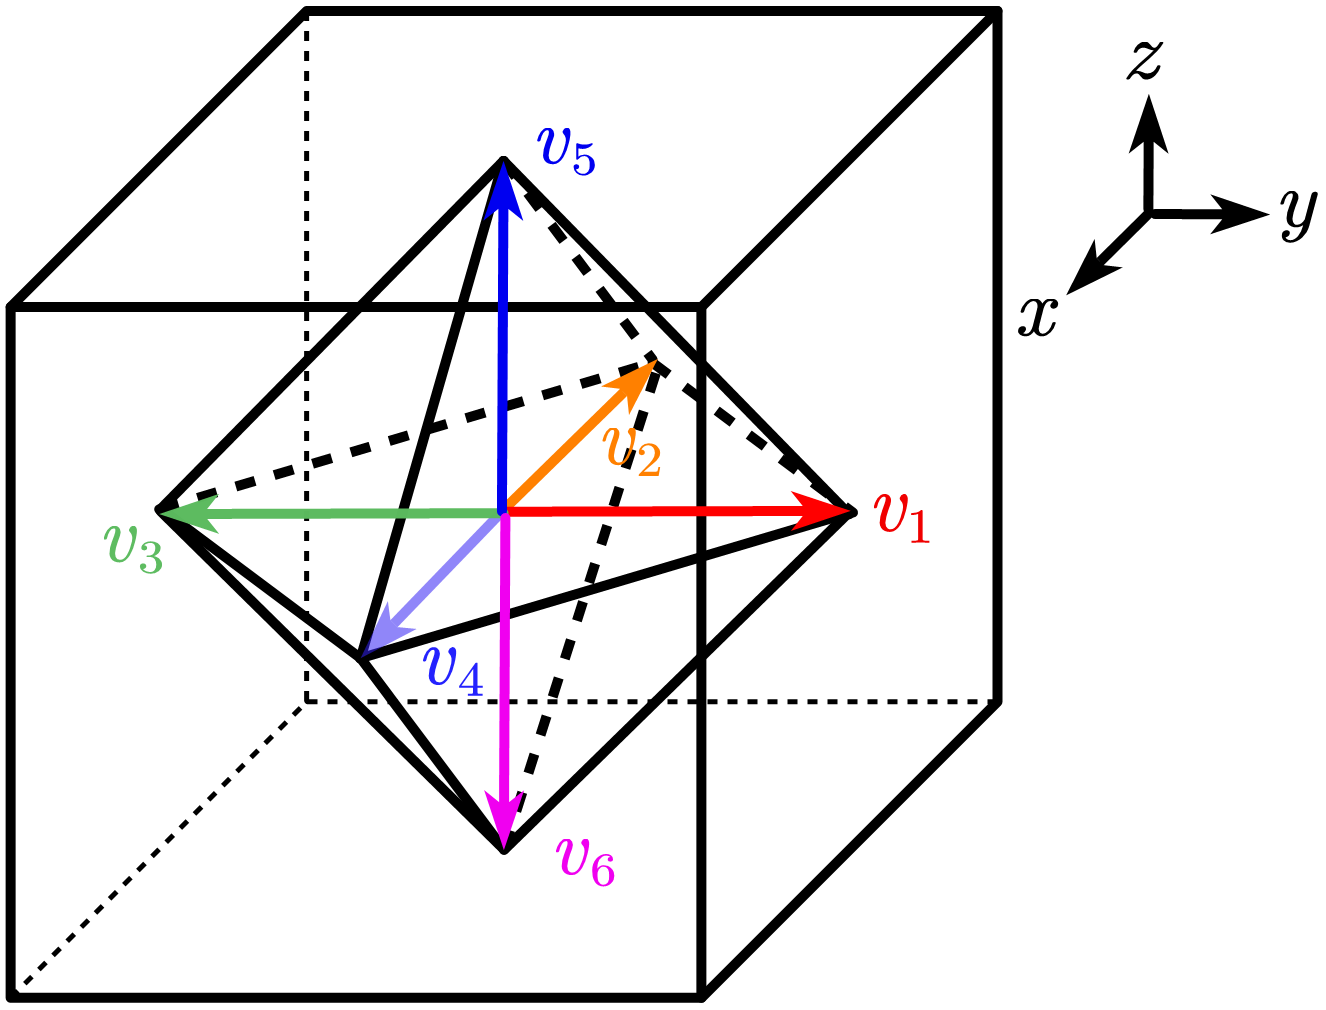
\includegraphics[scale=1.5]{./structures/exercise_2/octahedral.png}
		\captionof{figure}{A set of vectors $v_1$, $v_2$, $v_3$, $v_4$, $v_5$, and $v_6$ representing the six $\sigma$-hybrid orbitals used by the atom $\ce{A}$ to bond the six $\ce{B}$ atoms in $\ce{AB6}$.}\label{fig:octahedral}
		\end{center}
		\end{minipage}		
		
		The character table of the point group $\mathscr{O}_{\rm h}$ is shown below.		
		\begin{center}
		\begin{tabular}{ccccccccccccc}\hline
	$\mathscr{O}_{\rm h}$ & $E$ & $8C_3$ &	$3C_2$	& $6C_4$	&	$6C^\prime_2$	&	$i$	&	$8S_6$	&	$3\sigma_{h}$	&	$6S_4$ &	$6\sigma_{d}$	&	&\\ \hline
			$A_{1g}$	&	1	&	1	&	1	&	1	&	1	&	1	&	1	&	1	&	1	&	1	&		&	$x^2+y^2+z^2$\\
			$A_{2g}$	&	1	&	1	&	1	&	-1	&	-1	&	1	&	1	&	1	&	-1	&	-1	& 		&	\\
			$E_g$ 		&	2	&	-1	&	2	&	0	&	0	&	2	&	-1	&	2	&	0	&	0	& 		& ($2z^2-x^2-y^2$, $x^2-y^2$)\\
			$T_{1g}$	&	3	&	0	&	-1	&	1	&	-1	&	3	&	0	&	-1	&	1	&	-1	& ($R_x$, $R_y$, $R_z$)	&	\\
			$T_{2g}$ 	&	3	&	0	&	-1	&	-1	&	1	&	3	&	0	&	-1	&	-1	&	1	&		& ($xy$, $xz$, $yz$)\\
			$A_{1u}$	&	1	&	1	&	1	&	1	&	1	&	-1	&	-1	&	-1	&	-1	&	-1	&		&	\\4
			$A_{2u}$	&	1	&	1	&	1	&	-1	&	-1	&	-1	&	-1	&	-1	&	1	&	1	&		&	\\
			$E_u$ 		&	2	&	-1	&	2	&	0	&	0	&	-2	&	1	&	-2	&	0	&	0	& 		& \\ 
			$T_{1u}$	&	3	&	0	&	-1	&	1	&	-1	&	-3	&	0	&	1	&	-1	&	1	& ($x$, $y$, $z$)	&	\\
			$T_{2u}$ 	&	3	&	0	&	-1	&	-1	&	1	&	-3	&	0	&	1	&	1	&	-1	&		&	\\	\hline
		\end{tabular}
		\end{center}
		
		The character for $\Gamma^{\rm hyb}$ for the $\mathscr{O}_{\rm h}$ point group is 
		\begin{center}
		\begin{tabular}{ccccccccccc}\hline
	$\mathscr{O}_{\rm h}$ & $E$ & $8C_3$ &	$3C_2$	& $6C_4$	&	$6C^\prime_2$	&	$i$	&	$8S_6$	&	$3\sigma_{h}$	&	$6S_4$ &	$6\sigma_{d}$	\\ \hline
	$\chi^{\rm hyb}(C_i)$ & 6 & 0 & 2 & 2 & 0 &	0 & 0 & 4 & 0 & 2 \\ \hline
		\end{tabular}
		\end{center}
		
		\begin{equation*}
			\Gamma^{\rm hyb} = \Gamma^{A_{1g}} \oplus \Gamma^{E_g} \oplus \Gamma^{T_{1u}}.
		\end{equation*}
		
		\begin{center}
		\begin{tabular}{ccc} \hline
		$\Gamma^{A_{1g}}$	&	$\Gamma^{E_g}$	&	$\Gamma^{T_{1u}}$\\	\hline
		$\orbs$	&	($\orbd_{z^2}$, $\orbd_{x^2-y^2}$) & ($\orbp_x$, $\orbp_y$, $\orbp_z$) \\ \hline
		\end{tabular}
		\end{center}
		
		In conclusion, we have proved that for a molecule of octahedral symmetry the $\sigma$-bonding hybrid orbitals on the central atom are composed of six atomic orbitals, $\orbs$, $\orbp_x$, $\orbp_y$, $\orbp_z$, $\orbd_{z^2}$, and $\orbd_{x^2-y^2}$.
		
	\end{solution}
	
	\begin{exercise}
		Determine what type of $\pi$-bonding hybrid orbitals can be formed for the square planar $\ce{AB4}$ molecule which belongs to the $\mathscr{D}_{\rm 4h}$ point group.
	\end{exercise}
	
	\begin{solution}
		
		The character table of the point group $\mathscr{D}_{\rm 4h}$ is shown below.
		\begin{center}
		\begin{tabular}{ccccccccccccc}\hline
	$\mathscr{D}_{\rm 4h}$ & $E$ & $2C_4$ &	$C_2$	& $2C^\prime_2$	&	$2C^{\prime\prime}_2$	&	$i$	&	$2S_4$	&	$\sigma_{h}$	&	$2\sigma_{v}$ &	$2\sigma_{d}$	&		&\\ \hline
			$A_{1g}$	&	1	&	1	&	1	&	1	&	1	&	1	&	1	&	1	&	1	&	1	&		&	$x^2+y^2$; $z^2$\\
			$A_{2g}$	&	1	&	1	&	1	&	-1	&	-1	&	1	&	1	&	1	&	-1	&	-1	& $R_z$	&	\\
			$B_{1g}$	&	1	&	-1	&	1	&	1	&	-1	&	1	&	-1	&	1	&	1	&	-1	&		&	$x^2-y^2$\\
			$B_{2g}$ 	&	1	&	-1	&	1	&	-1	&	1	&	1	&	-1	&	1	&	-1	&	1	&		&	$xy$	\\
			$E_g$ 		&	2	&	0	&	-2	&	0	&	0	&	2	&	0	&	-2	&	0	&	0	& ($R_x$, $R_y$) & ($xz$, $yz$)\\ 
			$A_{1u}$	&	1	&	1	&	1	&	1	&	1	&	-1	&	-1	&	-1	&	-1	&	-1	&		&	\\
			$A_{2u}$	&	1	&	1	&	1	&	-1	&	-1	&	-1	&	-1	&	-1	&	1	&	1	&	$z$	&	\\
			$B_{1u}$	&	1	&	-1	&	1	&	1	&	-1	&	-1	&	1	&	-1	&	-1	&	1	&		&	\\
			$B_{2u}$ 	&	1	&	-1	&	1	&	-1	&	1	&	-1	&	1	&	-1	&	1	&	-1	&		&	\\
			$E_u$ 		&	2	&	0	&	-2	&	0	&	0	&	-2	&	0	&	2	&	0	&	0	& ($x$, $y$)	&\\ \hline
		\end{tabular}
		\end{center}
		
		\begin{minipage}[t]{1.0\linewidth}
		\begin{center}
		\setlength{\abovecaptionskip}{0.5em}
		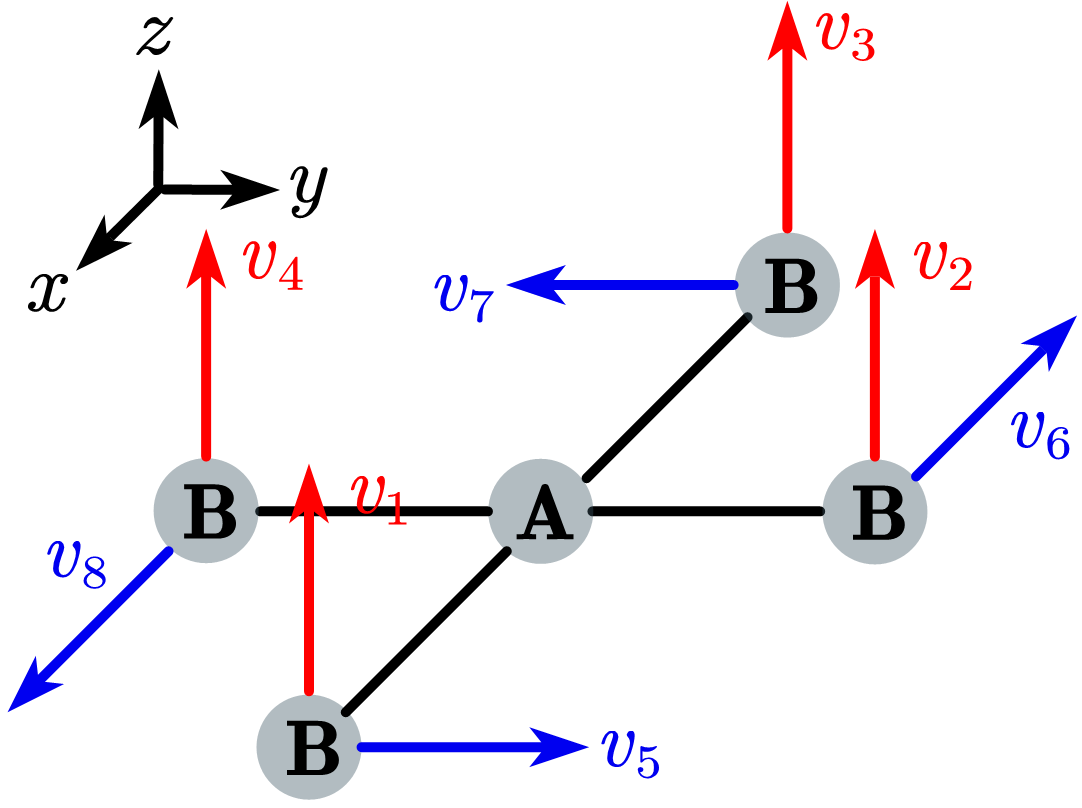
\includegraphics[scale=1.5]{./structures/exercise_3/square_planar.png}
		\captionof{figure}{rehstrjstfjs}
		\end{center}
		\end{minipage}	
		
		\begin{center}
		\begin{tabular}{ccccccccccccc}\hline
	$\mathscr{D}_{\rm 4h}$ & $E$ & $2C_4$ &	$C_2$	& $2C^\prime_2$	&	$2C^{\prime\prime}_2$	&	$i$	&	$2S_4$	&	$\sigma_{h}$	&	$2\sigma_{v}$ &	$2\sigma_{d}$	&		&\\ \hline
	$\chi^{\rm hyb}(C_i)$ & 8 & 0 & 0 & -4 & 0 & 0 & 0 & 0 & 0 & 0 \\
	$\chi^{\rm hyb}_{\rm perp}(C_i)$ & 4 & 0 & 0 & -2 & 0 & 0 & 0 & -4 & 2 & 0 \\ 
	$\chi^{\rm hyb}_{\rm plane}(C_i)$ & 4 & 0 & 0 & -2 & 0 & 0 & 0 & 4 & -2 & 0 \\ \hline
		\end{tabular}
		\end{center}
		
		\begin{align*}
			\Gamma^{\rm hyb}_{\rm perp} &= \Gamma^{A_{2u}} \oplus \Gamma^{B_{2u}} \oplus \Gamma^{E_g}, \\
			\Gamma^{\rm hyb}_{\rm plane} &= \Gamma^{A_{2g}} \oplus \Gamma^{B_{2g}} \oplus \Gamma^{E_u}.
		\end{align*}
		
		\begin{center}
		\begin{tabular}{ccc|ccc} \hline
		\multicolumn{3}{c|}{$\Gamma^{\rm hyb}_{\rm perp}$} & \multicolumn{3}{c}{$\Gamma^{\rm hyb}_{\rm plane}$} \\
		$\Gamma^{A_{2u}}$	&	$\Gamma^{B_{2u}}$	&	$\Gamma^{E_g}$	&	$\Gamma^{A_{2g}}$	&	$\Gamma^{B_{2g}}$	&	$\Gamma^{E_u}$	\\	\hline
		$\orbp_z$	&	none & ($\orbd_{xz}$, $\orbd_{yz}$)	&	none & $\orbd_{xy}$	&	($\orbp_x$, $\orbp_y$) \\ \hline
		\end{tabular}
		\end{center}
		
		Thus, we conclude two conclusions.
		\begin{itemize}
			
		\item There will be only 3 $\pi$-bonds which are formed by $\orbp_z$, $\orbd_{xz}$, and $\orbd_{yz}$, perpendicular to the molecular plane and they are shared equally amongst the 4 $\ce{B}$ atoms.
		
		\item There will be also only 3 $\pi$-bonds which are formed by $\orbd_{xy}$, $\orbp_x$, and $\orbp_y$, in the molecular plane and they are shared equally amongst the 4 $\ce{B}$ atoms.
		
		\end{itemize}
		
	\end{solution}
	
	\begin{exercise}
		Show that for the square planar $\ce{AB4}$ molecule a possible set of four $\sigma$-hybrid orbitals on A is composed of the atomic orbitals: $\orbs$, $\orbd_{x^2-y^2}$, $\orbp_x$, and $\orbp_y$. Find explicit expressions for the four hybrid orbitals.
	\end{exercise}
	
	\begin{solution}
		
		
				\begin{minipage}[t]{1.0\linewidth}
		\begin{center}
		\setlength{\abovecaptionskip}{0.5em}
		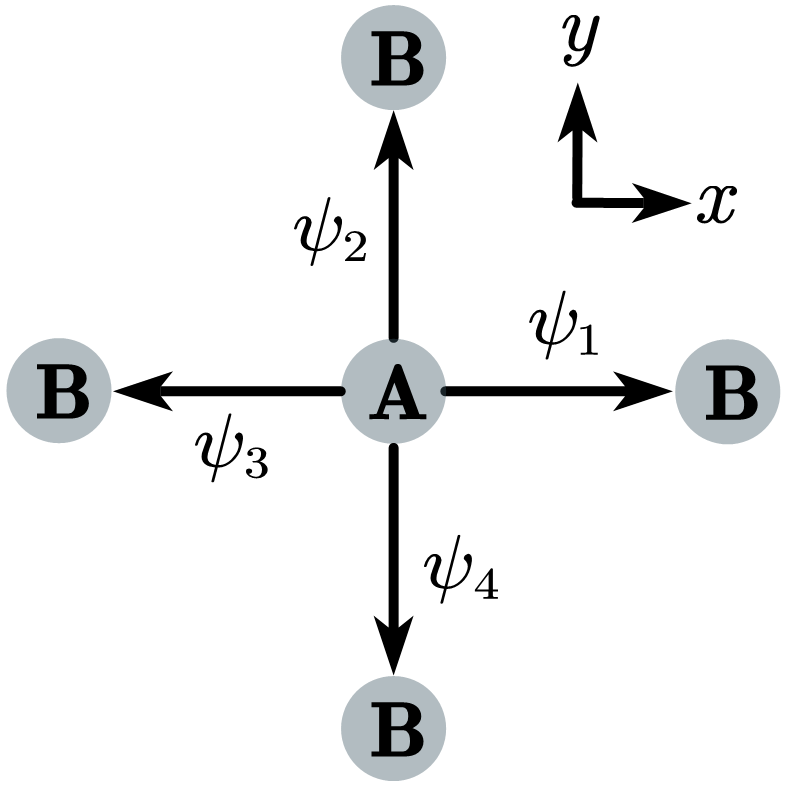
\includegraphics[scale=1.5]{./structures/exercise_4/square_planar.png}
		\captionof{figure}{fdsgfgsgh}
		\end{center}
		\end{minipage}	
		
	\end{solution}

\end{document}